\documentclass[a4,12pt]{article}
\usepackage{amsmath}
\usepackage{amssymb}
\usepackage[sorting=none]{biblatex}
\usepackage{hyperref}
\usepackage{graphicx}
\usepackage{subcaption}
% limit page margin
\usepackage[margin=1.2in]{geometry}

\addbibresource{reference.bib}
\graphicspath{{../figures/}}
\title{Proposal for PhD Research: 
Quantifying the Uncertainty in both On and Off-target Activity of Prime Editing}
\author{}
\date{}

\begin{document}

\maketitle

Prime editing is a novel editing 

My previous work on the master's thesis focused on the on target prediction of prime editing efficiency, however, the off-target activity of prime editing is still a major concern. 

With the recent development of a number of off-target site detection protocols supporting prime editors, it is now possible to quantify their off target activity using big data and deep learning techniques\parencite{liangGenomewideProfilingPrime2023,
zhuTrackingseqRevealsHeterogeneity2024}.

Although majority of the existing solution (including my master's thesis) was aiming at producing a point estimation as the predicted editing efficiency\parencite{mathisMachineLearningPrediction2024,yuPredictionEfficienciesDiverse2023,koeppelPredictionPrimeEditing2023}, the prime editing process itself can be viewed as a stochastic process due to the complexity of the physical processes involved. Thus, it could be more informative to model the posterior distribution of the activity of prime editing given the target loci and pegRNA sequence.

A reasonable starting point would be to investigate 

To validate this idea, I conducted some preliminary experiments on the on-target prediction of prime editing efficiency using the mathis et al's 90k PE2 HEK293T dataset\parencite{mathisPredictingPrimeEditing2023}.


Additional models including MC dropout/Deep ensemble

Thus, with the on and off target activity of prime editing quantified, we can provide a complete overview of the outcome of using a specific pegRNA sequence on a specific target loci. 

\begin{figure}
    \centering
    \begin{subfigure}{0.3\textwidth}
        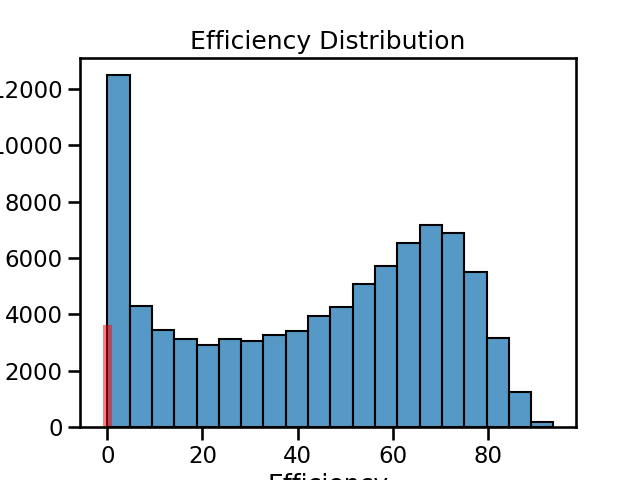
\includegraphics[width=\textwidth]{efficiency_distribution.png}
        \caption{Distribution of measured editing efficiency}
    \end{subfigure}
\end{figure}

\printbibliography

\end{document}